\documentclass[tikz]{standalone}
\usepackage{tikz}
\begin{document}
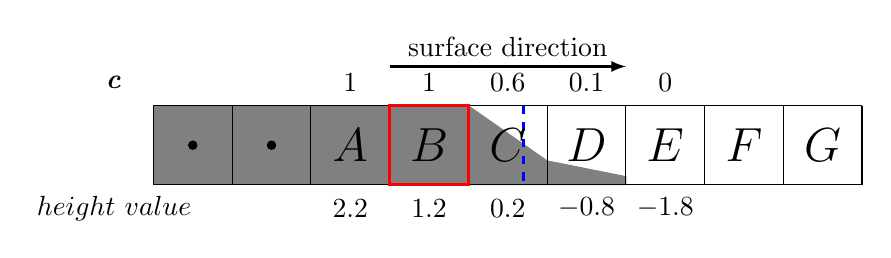
\begin{tikzpicture}[scale=1]
  \filldraw[gray] (-4.0,1)--(0,1)--(0,0)--(-4,0)--(-4.0,1);
  \filldraw[gray] (0.0,1)--(0,0)--(1,0)--(1,0.3)--(0,1);
  \filldraw[gray] (1.0,0.3)--(2,0.1)--(2,0)--(1,0)--(1,0.3);
  \draw[step=1cm] (-4.0,0) grid (5,1.0);
  \node at (-4.5,1.3) {\textbf{\emph{c}}};
  \node at (0.5,1.3) {$0.6$};
  \node at (-0.5,1.3) {$1$};
  \node at (1.5,1.3) {$0.1$};
  \node at (-1.5,1.3) {$1$};
  \node at (2.5,1.3) {$0$};
  \node at (-4.5,-0.3) {$height\ value$};
  \node at (0.5,-0.3) {$0.2$};
  \node at (-0.5,-0.3) {$1.2$};
  \node at (1.5,-0.3) {$-0.8$};
  \node at (-1.5,-0.3) {$2.2$};
  \node at (2.5,-0.3) {$-1.8$};
  \draw[very thick,dashed,blue] (0.7,1)--(0.7,0);
  \draw[very thick, red] (-1,0)--(-1,1)--(0,1)--(0,0)--cycle;
  \foreach \x in {-3.5,-2.5}
    \filldraw[] (\x,0.5) circle (1.5pt);
  \node at (-1.5,0.5) {\LARGE $A$};
  \node at (-0.5,0.5) {\LARGE $B$};
  \node at (0.5,0.5) {\LARGE $C$};
  \node at (1.5,0.5) {\LARGE $D$};
  \node at (2.5,0.5) {\LARGE $E$};
  \node at (3.5,0.5) {\LARGE $F$};
  \node at (4.5,0.5) {\LARGE $G$};
  \draw[thick,-latex] (-1,1.5)--(2,1.5) node[above,midway] {surface direction};
\end{tikzpicture}
\end{document}
